% answers.tex —— 2004 年·全国卷Ⅲ·文科 · 参考答案与详细解析片段
% 由 tools/generate_projects.py 依来源总账自 2004/2004_数学真题_全国3文_试题.md + 2004/2004_数学真题_全国3文_解析正文.md + 2004/2004_数学真题_全国3文_答案要点.md 生成，勿手改（改源 MD 后重跑）


\begin{gktip}
固定源 PDF 为印刷页码 192–193 的两页题面，不附答案。以下解析均依据固定源独立推导复算；第 21 题图形在 LaTeX 工程中以 TikZ/PGFPlots 矢量源重绘。
\end{gktip}

\begin{answer}
\gksolhead{1}{}

\textbf{题目}：

设集合 $M=\{(x,y)\mid x^2+y^2=1,x\in\mathbf{R},y\in\mathbf{R}\}$，$N=\{(x,y)\mid x^2-y=0,x\in\mathbf{R},y\in\mathbf{R}\}$，则集合 $M\cap N$ 中元素的个数为\mbox{（　　）}

（A）1　　（B）2　　（C）3　　（D）4

\Needspace{4\baselineskip}
\textbf{解析}

集合 $M=\{(x,y)\mid x^2+y^2=1,x\in\mathbf{R},y\in\mathbf{R}\}$ 表示单位圆；
集合 $N=\{(x,y)\mid x^2-y=0,x\in\mathbf{R},y\in\mathbf{R}\}$ 表示抛物线 $y=x^2$。
\Needspace{5\baselineskip}
联立两方程：
\nopagebreak[4]
\[
\begin{cases}
x^2+y^2=1,\\
x^2=y.
\end{cases}
\]
代入得 $y^2+y-1=0$，解得 $y=\dfrac{-1\pm\sqrt{5}}{2}$。
\Needspace{5\baselineskip}
因为抛物线要求 $y=x^2\geqslant 0$，所以负根舍去，仅有
\nopagebreak[4]
\[
y=\frac{\sqrt{5}-1}{2}\in(0,1).
\]
将此 $y$ 值代入 $x^2=y$，因为 $y>0$，方程有两个互异实数解 $x=\pm\sqrt{\dfrac{\sqrt{5}-1}{2}}$。
因此两曲线恰有两个交点，集合 $M\cap N$ 中元素的个数为 2。
故选 B。

\gkanswer{答案：B}

\end{answer}
\begin{answer}
\gksolhead{2}{}

\textbf{题目}：

函数 $y=\left|\sin\dfrac{x}{2}\right|$ 的最小正周期是\mbox{（　　）}

（A）$\dfrac{\pi}{2}$　　（B）$\pi$　　（C）$2\pi$　　（D）$4\pi$

\Needspace{4\baselineskip}
\textbf{解析}

函数 $y=\sin\dfrac{x}{2}$ 的周期为 $T_0=\dfrac{2\pi}{1/2}=4\pi$。
函数 $y=\left|\sin\dfrac{x}{2}\right|$ 将图像位于 $x$ 轴下方的部分对称翻折至 $x$ 轴上方，
\Needspace{5\baselineskip}
周期变为原周期的一半，即
\nopagebreak[4]
\[
T=\frac{4\pi}{2}=2\pi.
\]
故选 C。

\gkanswer{答案：C}

\end{answer}
\begin{answer}
\gksolhead{3}{}

\textbf{题目}：

记函数 $y=1+3^{-x}$ 的反函数为 $y=g(x)$，则 $g(10)=$\mbox{（　　）}

（A）2　　（B）$-2$　　（C）3　　（D）$-1$

\Needspace{4\baselineskip}
\textbf{解析}

设 $y=1+3^{-x}$。
\Needspace{5\baselineskip}
令 $y=10$，得
\nopagebreak[4]
\[
1+3^{-x}=10 \implies 3^{-x}=9=3^2.
\]
所以 $-x=2 \implies x=-2$。
由反函数的定义可知，$g(10)=-2$。
故选 B。

\gkanswer{答案：B}

\end{answer}
\begin{answer}
\gksolhead{4}{}

\textbf{题目}：

等比数列 $\{a_n\}$ 中，$a_2=9$，$a_5=243$，则 $\{a_n\}$ 的前 4 项和为\mbox{（　　）}

（A）81　　（B）120　　（C）168　　（D）192

\Needspace{4\baselineskip}
\textbf{解析}

在等比数列 $\{a_n\}$ 中，设公比为 $q$。
\Needspace{5\baselineskip}
由 $a_2=9$，$a_5=243$，得
\nopagebreak[4]
\[
q^3=\frac{a_5}{a_2}=\frac{243}{9}=27 \implies q=3.
\]
\Needspace{5\baselineskip}
首项为
\nopagebreak[4]
\[
a_1=\frac{a_2}{q}=\frac{9}{3}=3.
\]
\Needspace{5\baselineskip}
数列的前 4 项和为
\nopagebreak[4]
\[
S_4=\frac{a_1(1-q^4)}{1-q}=\frac{3(1-3^4)}{1-3}=\frac{3\times(-80)}{-2}=120.
\]
故选 B。

\gkanswer{答案：B}

\end{answer}
\begin{answer}
\gksolhead{5}{}

\textbf{题目}：

圆 $x^2+y^2-4x=0$ 在点 $P(1,\sqrt{3})$ 处的切线方程为\mbox{（　　）}

（A）$x+\sqrt{3}y-2=0$　　（B）$x+\sqrt{3}y-4=0$

（C）$x-\sqrt{3}y+4=0$　　（D）$x-\sqrt{3}y+2=0$

\Needspace{4\baselineskip}
\textbf{解析}

\Needspace{5\baselineskip}
将圆的方程配方得标准方程：
\nopagebreak[4]
\[
(x-2)^2+y^2=4,
\]
圆心为 $C(2,0)$，半径为 $r=2$。
将点 $P(1,\sqrt{3})$ 代入方程：$(1-2)^2+(\sqrt{3})^2=1+3=4$，点 $P$ 在圆上。
向量 $\overrightarrow{CP}=(1-2,\sqrt{3}-0)=(-1,\sqrt{3})$。
\Needspace{5\baselineskip}
因为切线与半径 $CP$ 垂直，故切线的斜率为
\nopagebreak[4]
\[
k=-\frac{1}{k_{CP}}=-\frac{1}{\frac{\sqrt{3}-0}{1-2}}=\frac{\sqrt{3}}{3}.
\]
\Needspace{5\baselineskip}
切线方程为
\nopagebreak[4]
\[
y-\sqrt{3}=\frac{\sqrt{3}}{3}(x-1) \implies \sqrt{3}x-3y+2\sqrt{3}=0 \implies x-\sqrt{3}y+2=0.
\]
故选 D。

\gkanswer{答案：D}

\end{answer}
\begin{answer}
\gksolhead{6}{}

\textbf{题目}：

$\left(\sqrt{x}-\dfrac{1}{x}\right)^6$ 展开式中的常数项为\mbox{（　　）}

（A）15　　（B）$-15$　　（C）20　　（D）$-20$

\Needspace{4\baselineskip}
\textbf{解析}

\Needspace{5\baselineskip}
二项式 $\left(\sqrt{x}-\dfrac{1}{x}\right)^6$ 展开式的通项为
\nopagebreak[4]
\[
T_{r+1}=\mathrm{C}_6^r (\sqrt{x})^{6-r}\left(-\frac{1}{x}\right)^r=(-1)^r \mathrm{C}_6^r x^{\frac{6-r}{2}-r}=(-1)^r \mathrm{C}_6^r x^{3-\frac{3}{2}r}.
\]
令指数为 0，即 $3-\dfrac{3}{2}r=0$，解得 $r=2$。
\Needspace{5\baselineskip}
常数项为
\nopagebreak[4]
\[
T_3=(-1)^2 \mathrm{C}_6^2=\frac{6\times 5}{2}=15.
\]
故选 A。

\gkanswer{答案：A}

\end{answer}
\begin{answer}
\gksolhead{7}{}

\textbf{题目}：

设复数 $z$ 的辐角主值为 $\dfrac{2\pi}{3}$，虚部为 $\sqrt{3}$，则 $z^2=$\mbox{（　　）}

（A）$-2-2\sqrt{3}\mathrm{i}$　　（B）$-2\sqrt{3}-2\mathrm{i}$

（C）$2+2\sqrt{3}\mathrm{i}$　　（D）$2\sqrt{3}+2\mathrm{i}$

\Needspace{4\baselineskip}
\textbf{解析}

设复数 $z=r(\cos\theta+\mathrm{i}\sin\theta)$（$r>0$）。
由题意，辐角主值 $\theta=\dfrac{2\pi}{3}$，虚部为 $r\sin\dfrac{2\pi}{3}=\sqrt{3}$。
\Needspace{5\baselineskip}
因为 $\sin\dfrac{2\pi}{3}=\dfrac{\sqrt{3}}{2}$，所以
\nopagebreak[4]
\[
r\cdot\frac{\sqrt{3}}{2}=\sqrt{3} \implies r=2.
\]
\Needspace{5\baselineskip}
复数 $z$ 为
\nopagebreak[4]
\[
z=2\left(\cos\frac{2\pi}{3}+\mathrm{i}\sin\frac{2\pi}{3}\right)=2\left(-\frac{1}{2}+\frac{\sqrt{3}}{2}\mathrm{i}\right)=-1+\sqrt{3}\mathrm{i}.
\]
\Needspace{5\baselineskip}
由棣莫弗公式，
\nopagebreak[4]
\[
z^2=r^2\left(\cos\frac{4\pi}{3}+\mathrm{i}\sin\frac{4\pi}{3}\right)=4\left(-\frac{1}{2}-\frac{\sqrt{3}}{2}\mathrm{i}\right)=-2-2\sqrt{3}\mathrm{i}.
\]
故选 A。

\gkanswer{答案：A}

\end{answer}
\begin{answer}
\gksolhead{8}{}

\textbf{题目}：

设双曲线的焦点在 $x$ 轴上，两条渐近线为 $y=\pm\dfrac{1}{2}x$，则该双曲线的离心率 $e=$\mbox{（　　）}

（A）5　　（B）$\sqrt{5}$　　（C）$\dfrac{\sqrt{5}}{2}$　　（D）$\dfrac{\sqrt{5}}{4}$

\Needspace{4\baselineskip}
\textbf{解析}

双曲线焦点在 $x$ 轴上，设其标准方程为 $\dfrac{x^2}{a^2}-\dfrac{y^2}{b^2}=1$（$a>0,b>0$）。
其渐近线方程为 $y=\pm\dfrac{b}{a}x$。
由题意，两条渐近线为 $y=\pm\dfrac{1}{2}x$，所以 $\dfrac{b}{a}=\dfrac{1}{2}$。
\Needspace{5\baselineskip}
离心率为
\nopagebreak[4]
\[
e=\frac{c}{a}=\sqrt{1+\left(\frac{b}{a}\right)^2}=\sqrt{1+\frac{1}{4}}=\frac{\sqrt{5}}{2}.
\]
故选 C。

\gkanswer{答案：C}

\end{answer}
\begin{answer}
\gksolhead{9}{}

\textbf{题目}：

不等式 $1<|x+1|<3$ 的解集为\mbox{（　　）}

（A）$(0,2)$　　（B）$(-2,0)\cup(2,4)$

（C）$(-4,0)$　　（D）$(-4,-2)\cup(0,2)$

\Needspace{4\baselineskip}
\textbf{解析}

\Needspace{5\baselineskip}
不等式 $1<|x+1|<3$ 等价于不等式组：
\nopagebreak[4]
\[
\begin{cases}
|x+1|>1,\\
|x+1|<3.
\end{cases}
\]
解 $|x+1|>1$ 得 $x+1>1$ 或 $x+1<-1$，即 $x>0$ 或 $x<-2$；
解 $|x+1|<3$ 得 $-3<x+1<3$，即 $-4<x<2$。
\Needspace{5\baselineskip}
两解集取交集，得
\nopagebreak[4]
\[
(-4,2)\cap\bigl((-\infty,-2)\cup(0,+\infty)\bigr)=(-4,-2)\cup(0,2).
\]
故选 D。

\gkanswer{答案：D}

\end{answer}
\begin{answer}
\gksolhead{10}{}

\textbf{题目}：

正三棱锥的底面边长为 2，侧面均为直角三角形，则此三棱锥的体积为\mbox{（　　）}

（A）$\dfrac{2\sqrt{2}}{3}$　　（B）$\sqrt{2}$　　（C）$\dfrac{\sqrt{2}}{3}$　　（D）$\dfrac{4\sqrt{2}}{3}$

\Needspace{4\baselineskip}
\textbf{解析}

设正三棱锥为 $P-ABC$，底面 $ABC$ 是边长为 2 的正三角形。
侧面均为直角三角形，由于正三棱锥各侧面为全等的等腰三角形，其顶角必为直角（若底角为直角则两底角均为 $90^\circ$，三角形内角和大于 $180^\circ$，不成立）。
即 $\angle APB=\angle BPC=\angle CPA=90^\circ$。
\Needspace{5\baselineskip}
设侧棱长为 $l$，在等腰直角三角形 $\triangle PAB$ 中，
\nopagebreak[4]
\[
l^2+l^2=2^2 \implies 2l^2=4 \implies l=\sqrt{2}.
\]
三条侧棱 $PA,PB,PC$ 两两垂直，三棱锥可以视为以 $\triangle PAB$ 为底面、$PC$ 为高的高立棱锥。
\Needspace{5\baselineskip}
体积为
\nopagebreak[4]
\[
V=\frac{1}{3}S_{\triangle PAB}\cdot PC=\frac{1}{3}\times\left(\frac{1}{2}\times\sqrt{2}\times\sqrt{2}\right)\times\sqrt{2}=\frac{\sqrt{2}}{3}.
\]
故选 C。

\gkanswer{答案：C}

\end{answer}
\begin{answer}
\gksolhead{11}{}

\textbf{题目}：

在 $\triangle ABC$ 中，$AB=3$，$BC=\sqrt{13}$，$AC=4$，则边 $AC$ 上的高为\mbox{（　　）}

（A）$\dfrac{3\sqrt{2}}{2}$　　（B）$\dfrac{3\sqrt{3}}{2}$　　（C）$\dfrac{3}{2}$　　（D）$3\sqrt{3}$

\Needspace{4\baselineskip}
\textbf{解析}

在 $\triangle ABC$ 中，$AB=3$，$BC=\sqrt{13}$，$AC=4$。
\Needspace{5\baselineskip}
由余弦定理，
\nopagebreak[4]
\[
\cos A=\frac{AB^2+AC^2-BC^2}{2AB\cdot AC}=\frac{3^2+4^2-(\sqrt{13})^2}{2\times 3\times 4}=\frac{9+16-13}{24}=\frac{12}{24}=\frac{1}{2}.
\]
因为 $A\in(0,\pi)$，所以 $A=60^\circ$。
$\sin A=\sin 60^\circ=\dfrac{\sqrt{3}}{2}$。
\Needspace{5\baselineskip}
边 $AC$ 上的高为
\nopagebreak[4]
\[
h=AB\sin A=3\times\frac{\sqrt{3}}{2}=\frac{3\sqrt{3}}{2}.
\]
故选 B。

\gkanswer{答案：B}

\end{answer}
\begin{answer}
\gksolhead{12}{}

\textbf{题目}：

将 4 名教师分配到 3 所中学任教，每所中学至少 1 名，则不同的分配方案共有\mbox{（　　）}

（A）12 种　　（B）24 种　　（C）36 种　　（D）48 种

\Needspace{4\baselineskip}
\textbf{解析}

将 4 名教师分配到 3 所中学任教，每所中学至少 1 名。
4 名教师分到 3 所学校，人数分组只能为 $2+1+1$。
\Needspace{5\baselineskip}
第一步，将 4 名教师分成人数为 2、1、1 的三个组，分组的方法数为
\nopagebreak[4]
\[
\frac{\mathrm{C}_4^2\mathrm{C}_2^1\mathrm{C}_1^1}{\mathrm{A}_2^2}=\frac{6\times 2\times 1}{2}=6.
\]
\Needspace{5\baselineskip}
第二步，将分好的 3 个组全排列分配到 3 所不同的中学，分配的方法数为
\nopagebreak[4]
\[
\mathrm{A}_3^3=6.
\]
\Needspace{5\baselineskip}
根据分步乘法计数原理，不同的分配方案共有
\nopagebreak[4]
\[
6\times 6=36\text{ \text{种}}.
\]
故选 C。

\gkanswer{答案：C}

\end{answer}
\begin{answer}
\gksolhead{13}{}

\textbf{题目}：

函数 $y=\sqrt{\log_{\frac{1}{2}}(x-1)}$ 的定义域是 $\underline{\hspace{3cm}}$。

\Needspace{4\baselineskip}
\textbf{解析}

\Needspace{5\baselineskip}
要使函数 $y=\sqrt{\log_{\frac{1}{2}}(x-1)}$ 有意义，需满足
\nopagebreak[4]
\[
\begin{cases}
x-1>0,\\
\log_{\frac{1}{2}}(x-1)\geqslant 0.
\end{cases}
\]
\Needspace{5\baselineskip}
由 $\log_{\frac{1}{2}}(x-1)\geqslant 0=\log_{\frac{1}{2}}1$，因为底数 $\dfrac{1}{2}\in(0,1)$，对数函数单调递减，所以
\nopagebreak[4]
\[
x-1\leqslant 1 \implies x\leqslant 2.
\]
又 $x-1>0 \implies x>1$。
综上，定义域为 $(1, 2]$。

\gkanswer{答案：$(1, 2]$}

\end{answer}
\begin{answer}
\gksolhead{14}{}

\textbf{题目}：

用平面 $\alpha$ 截半径为 $R$ 的球，如果球心到平面 $\alpha$ 的距离为 $\dfrac{R}{2}$，那么截得小圆的面积与球的表面积的比值为 $\underline{\hspace{3cm}}$。

\Needspace{4\baselineskip}
\textbf{解析}

球的半径为 $R$，球心到截面平面 $\alpha$ 的距离为 $d=\dfrac{R}{2}$。
\Needspace{5\baselineskip}
截得的小圆半径为
\nopagebreak[4]
\[
r=\sqrt{R^2-d^2}=\sqrt{R^2-\left(\frac{R}{2}\right)^2}=\frac{\sqrt{3}}{2}R.
\]
\Needspace{5\baselineskip}
截面小圆面积为
\nopagebreak[4]
\[
S_{\text{\text{圆}}}=\pi r^2=\frac{3}{4}\pi R^2.
\]
\Needspace{5\baselineskip}
球的表面积为
\nopagebreak[4]
\[
S_{\text{\text{球}}}=4\pi R^2.
\]
\Needspace{5\baselineskip}
两面积的比值为
\nopagebreak[4]
\[
\frac{S_{\text{\text{圆}}}}{S_{\text{\text{球}}}}=\frac{\frac{3}{4}\pi R^2}{4\pi R^2}=\frac{3}{16}.
\]

\gkanswer{答案：$\dfrac{3}{16}$}

\end{answer}
\begin{answer}
\gksolhead{15}{}

\textbf{题目}：

函数 $y=\sin x-\dfrac{1}{2}\cos x$（$x\in\mathbf{R}$）的最大值为 $\underline{\hspace{3cm}}$。

\Needspace{4\baselineskip}
\textbf{解析}

\Needspace{5\baselineskip}
应用辅助角公式，函数可化为
\nopagebreak[4]
\[
y=\sin x-\frac{1}{2}\cos x=\sqrt{1^2+\left(-\frac{1}{2}\right)^2}\sin(x+\varphi)=\frac{\sqrt{5}}{2}\sin(x+\varphi),
\]
其中 $\tan\varphi=-\dfrac{1}{2}$。
当 $\sin(x+\varphi)=1$ 时，函数取得最大值，最大值为 $\dfrac{\sqrt{5}}{2}$。

\gkanswer{答案：$\dfrac{\sqrt{5}}{2}$}

\end{answer}
\begin{answer}
\gksolhead{16}{}

\textbf{题目}：

设 $P$ 为圆 $x^2+y^2=1$ 上的动点，则点 $P$ 到直线 $3x-4y-10=0$ 的距离的最小值为 $\underline{\hspace{3cm}}$。

\Needspace{4\baselineskip}
\textbf{解析}

圆 $x^2+y^2=1$ 的圆心为坐标原点 $O(0,0)$，半径为 $r=1$。
\Needspace{5\baselineskip}
圆心到直线 $3x-4y-10=0$ 的距离为
\nopagebreak[4]
\[
d=\frac{|3\times 0-4\times 0-10|}{\sqrt{3^2+(-4)^2}}=\frac{10}{5}=2.
\]
因为 $d=2>r=1$，直线与圆相离。
\Needspace{5\baselineskip}
圆上的动点 $P$ 到直线的距离的最小值为
\nopagebreak[4]
\[
d_{\min}=d-r=2-1=1.
\]

\gkanswer{答案：$1$}

\end{answer}
\begin{answer}
\gksolhead{17}{}

\textbf{题目}：

（本小题满分 12 分）

解方程：$4^x-2^{x+2}-12=0$。

\Needspace{4\baselineskip}
\textbf{解析}

原方程为 $4^x-2^{x+2}-12=0$。
\Needspace{5\baselineskip}
因为 $4^x=(2^x)^2$，$2^{x+2}=4\cdot 2^x$，原方程可变形为
\nopagebreak[4]
\[
(2^x)^2-4\cdot 2^x-12=0.
\]
\Needspace{5\baselineskip}
令 $t=2^x$（$t>0$），方程化为关于 $t$ 的一元二次方程：
\nopagebreak[4]
\[
t^2-4t-12=0.
\]
\Needspace{5\baselineskip}
因式分解得
\nopagebreak[4]
\[
(t-6)(t+2)=0.
\]
解得 $t_1=6$，$t_2=-2$。
因为 $t=2^x>0$，所以 $t=-2$ 舍去，得 $2^x=6$。
\Needspace{5\baselineskip}
两边取以 2 为底的对数，得
\nopagebreak[4]
\[
x=\log_2 6\quad(\text{\text{或} } 1+\log_2 3).
\]

\gkanswer{答案：$x=\log_2 6$}

\end{answer}
\begin{answer}
\gksolhead{18}{}

\textbf{题目}：

（本小题满分 12 分）

已知 $\alpha$ 为锐角，且 $\tan\alpha=\dfrac{1}{2}$，求 $\dfrac{\sin 2\alpha\cos\alpha-\sin\alpha}{\sin 2\alpha\cos 2\alpha}$ 的值。

\Needspace{4\baselineskip}
\textbf{解析}

\Needspace{5\baselineskip}
化简待求式的分子：
\nopagebreak[4]
\[
\sin 2\alpha\cos\alpha-\sin\alpha=2\sin\alpha\cos^2\alpha-\sin\alpha=\sin\alpha(2\cos^2\alpha-1)=\sin\alpha\cos 2\alpha.
\]
\Needspace{5\baselineskip}
代入原式：
\nopagebreak[4]
\[
\frac{\sin 2\alpha\cos\alpha-\sin\alpha}{\sin 2\alpha\cos 2\alpha}=\frac{\sin\alpha\cos 2\alpha}{\sin 2\alpha\cos 2\alpha}=\frac{\sin\alpha}{\sin 2\alpha}=\frac{\sin\alpha}{2\sin\alpha\cos\alpha}=\frac{1}{2\cos\alpha}.
\]
\Needspace{5\baselineskip}
因为 $\alpha$ 为锐角且 $\tan\alpha=\dfrac{1}{2}$，由同角三角函数基本关系式：
\nopagebreak[4]
\[
\frac{1}{\cos^2\alpha}=1+\tan^2\alpha=1+\frac{1}{4}=\frac{5}{4} \implies \cos^2\alpha=\frac{4}{5}.
\]
因为 $\alpha$ 为锐角，所以 $\cos\alpha=\dfrac{2}{\sqrt{5}}=\dfrac{2\sqrt{5}}{5}$。
\Needspace{5\baselineskip}
因此，
\nopagebreak[4]
\[
\frac{1}{2\cos\alpha}=\frac{1}{2\times\frac{2\sqrt{5}}{5}}=\frac{\sqrt{5}}{4}.
\]

\gkanswer{答案：$\dfrac{\sqrt{5}}{4}$}

\end{answer}
\begin{answer}
\gksolhead{19}{}

\textbf{题目}：

（本小题满分 12 分）

设数列 $\{a_n\}$ 是公差不为零的等差数列，$S_n$ 是数列 $\{a_n\}$ 的前 $n$ 项和，且 $S_1^2=9S_2$，$S_4=4S_2$，求数列 $\{a_n\}$ 的通项公式。

\Needspace{4\baselineskip}
\textbf{解析}

设等差数列 $\{a_n\}$ 的公差为 $d$（$d\neq 0$），首项为 $a_1$。
前 $n$ 项和为 $S_n=na_1+\dfrac{n(n-1)}{2}d$。
\Needspace{5\baselineskip}
由题意：
\nopagebreak[4]
\[
S_1=a_1,\quad S_2=2a_1+d,\quad S_4=4a_1+6d.
\]
\Needspace{5\baselineskip}
已知 $S_4=4S_2$，即
\nopagebreak[4]
\[
4a_1+6d=4(2a_1+d)=8a_1+4d.
\]
\Needspace{5\baselineskip}
整理得
\nopagebreak[4]
\[
2d=4a_1 \implies d=2a_1.
\]
\Needspace{5\baselineskip}
又已知 $S_1^2=9S_2$，即
\nopagebreak[4]
\[
a_1^2=9(2a_1+d).
\]
\Needspace{5\baselineskip}
将 $d=2a_1$ 代入，得
\nopagebreak[4]
\[
a_1^2=9(2a_1+2a_1)=36a_1 \implies a_1(a_1-36)=0.
\]
若 $a_1=0$，则 $d=2a_1=0$，与题设公差 $d\neq 0$ 矛盾，故 $a_1\neq 0$。
因此 $a_1=36$。
公差 $d=2a_1=72$。
\Needspace{5\baselineskip}
所以数列 $\{a_n\}$ 的通项公式为
\nopagebreak[4]
\[
a_n=a_1+(n-1)d=36+72(n-1)=72n-36.
\]

\gkanswer{答案：$a_n=72n-36$}

\end{answer}
\begin{answer}
\gksolhead{20}{}

\textbf{题目}：

（本小题满分 12 分）

某村计划建造一个室内面积为 $800\text{ m}^2$ 的矩形蔬菜温室。在温室内，沿左、右两侧与后侧内墙各保留 $1\text{ m}$ 宽的通道，沿前侧内墙保留 $3\text{ m}$ 宽的空地。当矩形温室的边长各为多少时，蔬菜的种植面积最大？最大种植面积是多少？

\Needspace{4\baselineskip}
\textbf{解析}

设矩形温室前后两侧内墙的边长为 $x\text{ m}$，左右两侧内墙的边长为 $y\text{ m}$（$x>0,y>0$）。
\Needspace{5\baselineskip}
由题意，温室的室内面积为
\nopagebreak[4]
\[
xy=800.
\]
在温室内：
左右两侧各保留 $1\text{ m}$ 通道，蔬菜种植区域横向长为 $x-2\text{ m}$（需 $x>2$）；
后侧保留 $1\text{ m}$ 通道，前侧保留 $3\text{ m}$ 空地，蔬菜种植区域纵向长为 $y-(1+3)=y-4\text{ m}$（需 $y>4$）。
\Needspace{5\baselineskip}
蔬菜种植面积为
\nopagebreak[4]
\[
S=(x-2)(y-4)=xy-4x-2y+8.
\]
\Needspace{5\baselineskip}
将 $y=\dfrac{800}{x}$ 代入，得
\nopagebreak[4]
\[
S=800-4x-2\cdot\frac{800}{x}+8=808-\left(4x+\frac{1600}{x}\right).
\]
\Needspace{5\baselineskip}
因为 $x>2$，由基本不等式：
\nopagebreak[4]
\[
4x+\frac{1600}{x}\geqslant 2\sqrt{4x\cdot\frac{1600}{x}}=2\sqrt{6400}=160,
\]
当且仅当 $4x=\dfrac{1600}{x} \implies x^2=400 \implies x=20$ 时等号成立。
此时 $y=\dfrac{800}{20}=40$。
\Needspace{5\baselineskip}
最大种植面积为
\nopagebreak[4]
\[
S_{\max}=808-160=648\text{ m}^2.
\]
答：当矩形温室前后两侧内墙边长为 $20\text{ m}$，左右两侧内墙边长为 $40\text{ m}$ 时，蔬菜的种植面积最大，最大种植面积是 $648\text{ m}^2$。

\gkanswer{答案：当温室前后两侧边长为 $20\text{ m}$，左右两侧边长为 $40\text{ m}$ 时，蔬菜的种植面积最大，最大面积为 $648\text{ m}^2$}

\end{answer}
\begin{answer}
\gksolhead{21}{}

\textbf{题目}：

（本小题满分 12 分）

三棱锥 $P-ABC$ 中，侧面 $PAC$ 与底面 $ABC$ 垂直，$PA=PB=PC=3$。
\nopagebreak[4]
\begin{center}% 2004 年全国卷Ⅲ文科第 21 题：三棱锥立体几何图
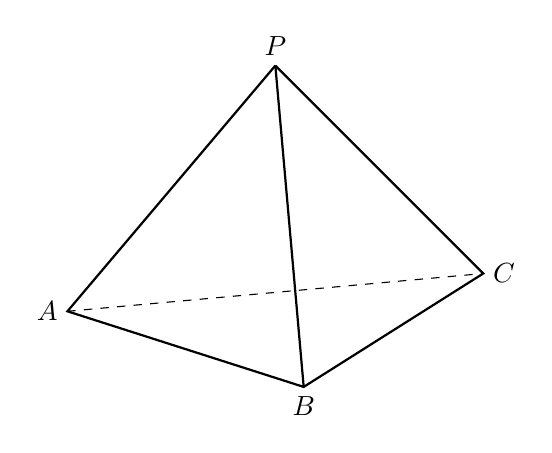
\begin{tikzpicture}[>=stealth,scale=1.2]
  % Coordinates
  \coordinate (A) at (-2.2,-0.4);
  \coordinate (B) at (0.3,-1.2);
  \coordinate (C) at (2.2,0);
  \coordinate (P) at (0,2.2);

  % Edges
  \draw[thick] (P) -- (A) -- (B) -- (C) -- (P);
  \draw[thick] (P) -- (B);
  \draw[dashed] (A) -- (C);

  % Labels
  \node[left] at (A) {$A$};
  \node[below] at (B) {$B$};
  \node[right] at (C) {$C$};
  \node[above] at (P) {$P$};
\end{tikzpicture}
\end{center}
\nopagebreak[4]
（1）求证：$AB\perp BC$；

（2）设 $AB=BC=2\sqrt{3}$，求 $AC$ 与平面 $PBC$ 所成角的大小。

\Needspace{4\baselineskip}
\textbf{解析}

（1）\textbf{证明}：
取 $AC$ 的中点 $D$，连接 $PD$、$BD$。
因为 $PA=PC=3$，$D$ 为 $AC$ 中点，所以 $PD\perp AC$。
又因为侧面 $PAC\perp$ 底面 $ABC$，平面 $PAC\cap$ 平面 $ABC=AC$，$PD\subset$ 平面 $PAC$ 且 $PD\perp AC$，
所以 $PD\perp$ 底面 $ABC$。
因此 $PD\perp BD$。
在直角三角形 $\triangle PDB$ 中，$PB^2=PD^2+BD^2$；
在直角三角形 $\triangle PDA$ 中，$PA^2=PD^2+AD^2$。
\Needspace{5\baselineskip}
已知 $PA=PB=3$，所以
\nopagebreak[4]
\[
PD^2+AD^2=PD^2+BD^2 \implies BD=AD.
\]
因为 $D$ 是 $AC$ 的中点，所以 $AD=CD=\dfrac{1}{2}AC$，
从而 $BD=\dfrac{1}{2}AC$。
在 $\triangle ABC$ 中，中线 $BD$ 的长等于边 $AC$ 的一半，
所以 $\triangle ABC$ 是以 $AC$ 为斜边的直角三角形，即 $\angle ABC=90^\circ$，
故 $AB\perp BC$。

（2）\textbf{求 $AC$ 与平面 $PBC$ 所成角的大小}：
在等腰直角三角形 $\triangle ABC$ 中，$AB=BC=2\sqrt{3}$，
斜边 $AC=\sqrt{AB^2+BC^2}=2\sqrt{6}$，
中点 $D$ 满足 $AD=DC=BD=\sqrt{6}$，且 $BD\perp AC$。
\Needspace{5\baselineskip}
在直角三角形 $\triangle PDA$ 中，
\nopagebreak[4]
\[
PD=\sqrt{PA^2-AD^2}=\sqrt{3^2-(\sqrt{6})^2}=\sqrt{3}.
\]
建立空间直角坐标系：以 $D$ 为原点，射线 $DA$ 为 $x$ 轴正方向，射线 $DB$ 为 $y$ 轴正方向，射线 $DP$ 为 $z$ 轴正方向。
\Needspace{5\baselineskip}
各点坐标为：
\nopagebreak[4]
\[
D(0,0,0),\quad A(\sqrt{6},0,0),\quad C(-\sqrt{6},0,0),\quad B(0,\sqrt{6},0),\quad P(0,0,\sqrt{3}).
\]
向量 $\overrightarrow{AC}=(-2\sqrt{6},0,0)$，其模长 $|\overrightarrow{AC}|=2\sqrt{6}$。
\Needspace{5\baselineskip}
平面 $PBC$ 的两个方向向量为：
\nopagebreak[4]
\[
\overrightarrow{BC}=(-\sqrt{6},-\sqrt{6},0),\quad \overrightarrow{BP}=(0,-\sqrt{6},\sqrt{3}).
\]
\Needspace{5\baselineskip}
设平面 $PBC$ 的法向量为 $\boldsymbol{n}=(x,y,z)$，则
\nopagebreak[4]
\[
\begin{cases}
\boldsymbol{n}\cdot\overrightarrow{BC}=-\sqrt{6}x-\sqrt{6}y=0,\\
\boldsymbol{n}\cdot\overrightarrow{BP}=-\sqrt{6}y+\sqrt{3}z=0.
\end{cases}
\]
解得 $y=-x$，$z=-\sqrt{2}x$。
取 $x=1$，得法向量 $\boldsymbol{n}=(1,-1,-\sqrt{2})$，模长 $|\boldsymbol{n}|=2$。
\Needspace{5\baselineskip}
设直线 $AC$ 与平面 $PBC$ 所成角为 $\theta$（$\theta\in[0,\pi/2]$），则
\nopagebreak[4]
\[
\sin\theta=|\cos\langle\boldsymbol{n},\overrightarrow{AC}\rangle|=\frac{|\boldsymbol{n}\cdot\overrightarrow{AC}|}{|\boldsymbol{n}||\overrightarrow{AC}|}=\frac{|1\times(-2\sqrt{6})|}{2\times 2\sqrt{6}}=\frac{2\sqrt{6}}{4\sqrt{6}}=\frac{1}{2}.
\]
因为 $\theta\in[0,\pi/2]$，所以 $\theta=30^\circ$（即 $\dfrac{\pi}{6}$）。
故 $AC$ 与平面 $PBC$ 所成角的大小为 $30^\circ$（或 $\dfrac{\pi}{6}$）。

\gkanswer{答案：（1）证明见解析；（2）$30^\circ$（或 $\dfrac{\pi}{6}$）}

\end{answer}
\begin{answer}
\gksolhead{22}{}

\textbf{题目}：

（本小题满分 14 分）

设椭圆 $\dfrac{x^2}{m+1}+y^2=1$ 的两个焦点是 $F_1(-c,0)$ 与 $F_2(c,0)$（$c>0$），且椭圆上存在一点 $P$，使得直线 $PF_1$ 与 $PF_2$ 垂直。

（1）求实数 $m$ 的取值范围；

（2）设 $L$ 是相应于焦点 $F_2$ 的准线，直线 $PF_2$ 与 $L$ 相交于点 $Q$，若 $\dfrac{|QF_2|}{|PF_2|}=2-\sqrt{3}$，求直线 $PF_2$ 的方程。

\Needspace{4\baselineskip}
\textbf{解析}

椭圆方程为 $\dfrac{x^2}{m+1}+y^2=1$，焦点 $F_1(-c,0)$ 与 $F_2(c,0)$（$c>0$）在 $x$ 轴上。
所以 $a^2=m+1$，$b^2=1$。
因为焦点在 $x$ 轴上，所以 $a^2>b^2 \implies m+1>1 \implies m>0$。
半焦距 $c=\sqrt{a^2-b^2}=\sqrt{m}$。

（1）\textbf{求实数 $m$ 的取值范围}：
由题意，椭圆上存在点 $P$，使得 $PF_1\perp PF_2$。
在直角三角形 $\triangle PF_1F_2$ 中，$F_1F_2$ 为斜边，其斜边中点为坐标原点 $O$。
由直角三角形斜边中线定理，$|OP|=\dfrac{1}{2}|F_1F_2|=c$。
即点 $P$ 既在椭圆上，又在以原点为圆心、半径为 $c$ 的圆 $x^2+y^2=c^2=m$ 上。
\Needspace{5\baselineskip}
由椭圆方程得 $x^2=(m+1)(1-y^2)$，代入圆的方程：
\nopagebreak[4]
\[
(m+1)(1-y^2)+y^2=m \implies m+1-my^2=m \implies my^2=1.
\]
因为 $m>0$，所以 $y^2=\dfrac{1}{m}$。
椭圆上点的纵坐标满足 $y\in[-1,1]$，即 $y^2\leqslant 1$。
\Needspace{5\baselineskip}
所以
\nopagebreak[4]
\[
\frac{1}{m}\leqslant 1 \implies m\geqslant 1.
\]
当 $m\geqslant 1$ 时，$y^2=\dfrac{1}{m}\in(0,1]$，对应的 $x^2=(m+1)\left(1-\dfrac{1}{m}\right)=\dfrac{m^2-1}{m}\geqslant 0$，存在实数坐标满足条件。
故实数 $m$ 的取值范围是 $m\geqslant 1$（或 $[1,+\infty)$）。

（2）\textbf{求直线 $PF_2$ 的方程}：
相应于焦点 $F_2(c,0)$ 的准线 $L$ 的方程为 $x=\dfrac{a^2}{c}$。
\Needspace{5\baselineskip}
焦点 $F_2(c,0)$ 到准线 $L$ 的距离为
\nopagebreak[4]
\[
d=\frac{a^2}{c}-c=\frac{a^2-c^2}{c}=\frac{b^2}{c}=\frac{1}{\sqrt{m}}.
\]
设直线 $PF_2$ 的倾斜角为 $\alpha$（$\alpha\neq 90^\circ$）。
在以 $F_2$、准线交点 $Q$ 和 $F_2$ 在准线上的射影 $F_0$ 构成的直角三角形中，$F_2F_0\perp L$。
\Needspace{5\baselineskip}
直线 $PF_2$ 与准线相交于点 $Q$，易得
\nopagebreak[4]
\[
|QF_2|=\frac{d}{|\cos\alpha|}=\frac{b^2}{c|\cos\alpha|}=\frac{1}{\sqrt{m}|\cos\alpha|}.
\]
在直角三角形 $\triangle PF_1F_2$ 中，$PF_1\perp PF_2$，$F_1F_2=2c$ 为斜边。
\Needspace{5\baselineskip}
直线 $F_1F_2$ 位于 $x$ 轴上，所以直角边 $PF_2$ 与 $x$ 轴方向所夹角的余弦值为
\nopagebreak[4]
\[
|\cos\alpha|=\cos\angle PF_2F_1=\frac{|PF_2|}{2c}.
\]
\Needspace{5\baselineskip}
将 $|\cos\alpha|=\dfrac{|PF_2|}{2c}$ 代入 $|QF_2|$ 的表达式，得
\nopagebreak[4]
\[
|QF_2|=\frac{b^2}{c\cdot\frac{|PF_2|}{2c}}=\frac{2b^2}{|PF_2|}=\frac{2}{|PF_2|}.
\]
\Needspace{5\baselineskip}
因此，
\nopagebreak[4]
\[
\frac{|QF_2|}{|PF_2|}=\frac{2}{|PF_2|^2}.
\]
\Needspace{5\baselineskip}
已知 $\dfrac{|QF_2|}{|PF_2|}=2-\sqrt{3}$，所以
\nopagebreak[4]
\[
\frac{2}{|PF_2|^2}=2-\sqrt{3} \implies |PF_2|^2=\frac{2}{2-\sqrt{3}}=2(2+\sqrt{3})=4+2\sqrt{3}=(\sqrt{3}+1)^2.
\]
\Needspace{5\baselineskip}
解得
\nopagebreak[4]
\[
|PF_2|=\sqrt{3}+1.
\]
\Needspace{5\baselineskip}
在直角三角形 $\triangle PF_1F_2$ 中，由椭圆的第一定义：
\nopagebreak[4]
\[
(|PF_1|+|PF_2|)^2=(2a)^2=4a^2.
\]
\Needspace{5\baselineskip}
展开得
\nopagebreak[4]
\[
|PF_1|^2+|PF_2|^2+2|PF_1||PF_2|=4c^2+2|PF_1||PF_2|=4a^2,
\]
\Needspace{5\baselineskip}
所以
\nopagebreak[4]
\[
|PF_1||PF_2|=2(a^2-c^2)=2b^2=2.
\]
\Needspace{5\baselineskip}
从而
\nopagebreak[4]
\[
|PF_1|=\frac{2}{|PF_2|}=\frac{2}{\sqrt{3}+1}=\sqrt{3}-1.
\]
\Needspace{5\baselineskip}
在直角三角形 $\triangle PF_1F_2$ 中，由勾股定理：
\nopagebreak[4]
\[
4c^2=|PF_1|^2+|PF_2|^2=(\sqrt{3}-1)^2+(\sqrt{3}+1)^2=(4-2\sqrt{3})+(4+2\sqrt{3})=8,
\]
解得 $c^2=2$，即 $c=\sqrt{2}$。
因为 $c=\sqrt{m}$，所以 $m=2$（满足 $m\geqslant 1$）。
焦点 $F_2$ 的坐标为 $(\sqrt{2},0)$。
因为 $|PF_1|=\sqrt{3}-1<|PF_2|=\sqrt{3}+1$，所以点 $P$ 的横坐标小于 0（$P$ 在 $y$ 轴左侧）。
\Needspace{5\baselineskip}
在直角三角形 $\triangle PF_1F_2$ 中，
\nopagebreak[4]
\[
\cos\angle PF_2F_1=\frac{|PF_2|}{2c}=\frac{\sqrt{3}+1}{2\sqrt{2}}=\frac{\sqrt{6}+\sqrt{2}}{4}=\cos 15^\circ.
\]
所以 $\angle PF_2F_1=15^\circ$。
因为焦点 $F_1$ 位于 $F_2(\sqrt{2},0)$ 的左侧，直线 $PF_2$ 与 $x$ 轴正方向的夹角为 $180^\circ\pm 15^\circ$。
\Needspace{5\baselineskip}
直线 $PF_2$ 的斜率为
\nopagebreak[4]
\[
k=\tan(180^\circ\pm 15^\circ)=\mp\tan 15^\circ=\mp(2-\sqrt{3}).
\]
\Needspace{5\baselineskip}
又直线经过点 $F_2(\sqrt{2},0)$，直线方程为
\nopagebreak[4]
\[
y=\mp(2-\sqrt{3})(x-\sqrt{2}),
\]
\Needspace{5\baselineskip}
整理得
\nopagebreak[4]
\[
(2-\sqrt{3})x-y-(2\sqrt{2}-\sqrt{6})=0\quad\text{\text{或}}\quad (2-\sqrt{3})x+y-(2\sqrt{2}-\sqrt{6})=0.
\]

\gkanswer{答案：（1）$m\geqslant 1$；（2）$(2-\sqrt{3})x-y-(2\sqrt{2}-\sqrt{6})=0$ 或 $(2-\sqrt{3})x+y-(2\sqrt{2}-\sqrt{6})=0$}

\end{answer}